\documentclass[letterpaper,10pt,conference]{ieeeconf}

% Copy the current ICRA 2027 template files from PaperPlaza into this directory.
\IEEEoverridecommandlockouts
\overrideIEEEmargins

\usepackage{amsmath,amssymb}
\usepackage{booktabs}
\usepackage{graphicx}
\usepackage{microtype}
\usepackage{url}

\title{\LARGE \bf
When Can Humans Really Intervene?\\
Capacity-Aware Safety Guarantees for Supervisory Multi-Robot Systems
}

\author{Anonymous Authors}

\begin{document}
\maketitle
\thispagestyle{empty}
\pagestyle{empty}

\begin{abstract}
Human-in-the-loop architectures are often treated as if providing an intervention channel were sufficient to preserve human control. This paper shows that such a guarantee is inherently system-level: escalation quality, event base rates, finite supervisory capacity, human processing time, intervention deadlines, and correlated demand jointly determine whether intervention remains practically available. We define effective human control (EHC) as the probability that an oversight-critical event is escalated, reviewed correctly, and acted upon before its deadline. An analytically tractable multi-server baseline yields a deadline-aware control capacity and four consequences. First, some targets are infeasible regardless of staffing because human service time itself imposes a hard ceiling. Second, increasing escalation sensitivity can reduce EHC when additional false alerts create sufficient congestion. Third, in rare-event regimes any fixed nonzero false-positive rate induces a first-order staffing requirement linear in fleet scale. Fourth, average utilization cannot guarantee EHC under synchronized alert bursts. The framework recovers classical fan-out as a special stability case. Dimensionless simulations with non-Poisson arrivals and non-exponential service distributions show that the main effects persist beyond the analytical assumptions.
\end{abstract}

\section{Introduction}

Many autonomous-system designs use the same safety pattern: routine decisions are delegated to automation while sensitive situations are escalated to a human supervisor. Yet the existence of an escalation mechanism and an override interface does not imply that a human can actually intervene when needed. A critical alert can be missed by the escalation mechanism, delayed behind nuisance alerts, arrive during a common-cause burst, or require more human processing time than the available deadline permits.

We therefore treat human control as an end-to-end performance property. Let \(Z=1\) denote an oversight-critical situation. We define
\begin{equation}
C=P(\text{successful timely human intervention}\mid Z=1),
\label{eq:ehc}
\end{equation}
and ask when a supervisory architecture can guarantee \(C\ge C_{\min}\).

Our contribution is not a new queueing model, fan-out metric, or false-alarm concept. Instead, we connect escalation reliability, base rates, finite human capacity, and deadlines in one guarantee. This yields four system-level results:
\begin{enumerate}
    \item a deadline-aware feasibility ceiling and unique alert-rate capacity for a finite operator pool;
    \item an \emph{Oversight Paradox}, in which increasing escalation sensitivity can reduce end-to-end control;
    \item a rare-event scaling law showing that fixed nonzero false-positive rates induce staffing linear in fleet scale;
    \item a proof that equal average utilization can produce arbitrarily different deadline-constrained control under synchronized demand.
\end{enumerate}
We additionally recover classical potential fan-out as a special stability case and evaluate robustness under non-Poisson arrivals and non-exponential service times.

\section{Related Work}
\label{sec:related}

\textbf{Supervisory capacity and fan-out.}
Human--multi-robot supervision has long been modeled in terms of neglect or self-sufficiency time, interaction time, and the resulting number of agents that one operator can sustain. Cummings and Mitchell explicitly modeled interaction waiting, queueing, and situation-awareness costs in multi-UAV supervision \cite{cummings2008capacity}, while Savla and Frazzoli treated human task management as a dynamical queue whose service rate depends on workload \cite{savla2012queue}. Most recently, Perkins et al. revisited fan-out by separating robot self-sufficiency from the human's estimate of that self-sufficiency \cite{perkins2025fanout}. We use these results as capacity baselines rather than novelty claims; in fact, our stability condition recovers potential fan-out as a special case.

\textbf{Alerts, querying, and human effort.}
Alert design can improve or degrade supervisory decisions. Al-Hussaini et al. evaluate alert generation and tasking suggestions in multi-robot search-and-rescue missions \cite{alhussaini2024alerts}. Recent HITL robotics also explicitly trades robot uncertainty against the cost of querying humans: Banerjee et al. use calibrated uncertainty and human intervention cost to decide when modular robot policies should request help \cite{banerjee2026failure}. These approaches optimize or evaluate when to ask for human input. Our question is complementary: given an escalation policy, finite shared human capacity, base rates, and deadlines, when does the resulting architecture provide a specified end-to-end probability of effective intervention?

\textbf{Meaningful human control.}
Meaningful human control (MHC) work emphasizes that nominal involvement is insufficient. Verhagen et al. operationalize MHC for variable-autonomy firefighting teams and identify operator overload as a threat to control \cite{verhagen2024mhc}; Prinz and Mathew further translate MHC into HRI interface-design requirements \cite{prinz2026operationalizing}. We provide a quantitative system-level counterpart: a probabilistic guarantee connecting referral accuracy to the finite supervisory channel and the time available to act.

\section{Model}
\label{sec:model}

A fleet of \(N\) agents generates candidate supervisory situations at rate
\begin{equation}
\Lambda=N\lambda.
\end{equation}
A situation is oversight-critical with probability \(\pi\). Let \(R=1\) denote referral to a human. The escalation mechanism has
\begin{equation}
r=P(R=1\mid Z=1),\qquad
f=P(R=1\mid Z=0).
\end{equation}
Under independent thinning, human alerts arrive at rate
\begin{equation}
\nu=\Lambda[\pi r+(1-\pi)f].
\label{eq:alert-rate}
\end{equation}

There are \(M\) pooled operators. In the analytical baseline, alerts are FCFS and human service times are iid exponential with rate \(\mu\). Let \(W\) be queue waiting time, \(S\) service time, and \(D\) the intervention deadline. Define
\begin{equation}
Q_M(\nu,D)=P(W+S\le D).
\end{equation}
If \(h\) is the probability of a correct human response after timely review and \(a\) the probability that the correct action successfully takes effect, then
\begin{equation}
\boxed{C=rhaQ_M(\nu,D).}
\label{eq:main}
\end{equation}

Let \(m=E[S]\) and define
\begin{equation}
A=\nu m,\qquad
d=\frac{D}{m},\qquad
\rho=\frac{A}{M}.
\label{eq:dimensionless}
\end{equation}
For the M/M/\(M\) baseline, \(Q_M\) depends on physical units only through \((A,d,M)\).

\section{Effective-Control Guarantees}
\label{sec:theory}

\subsection{Feasibility and capacity}

\textbf{Theorem 1 (service-time ceiling).}
For any nonnegative waiting time and any human service-time distribution \(S\),
\begin{equation}
\boxed{C\le rha\,P(S\le D).}
\end{equation}
Thus a target exceeding this bound is impossible regardless of staffing or scheduling.

\emph{Proof sketch:} completion requires \(W+S\le D\), while \(W\ge0\), hence \(\{W+S\le D\}\subseteq\{S\le D\}\).

For exponential service this gives \(C\le rha(1-e^{-\mu D})\).

\textbf{Theorem 2 (effective-control capacity).}
For fixed \(M,\mu,D\), the stationary M/M/\(M\) completion probability is continuous and strictly decreasing in \(\nu\), from \(1-e^{-\mu D}\) at zero load to zero as \(\nu\uparrow M\mu\). Therefore every feasible target defines a unique \(\nu_M^*\) satisfying
\begin{equation}
Q_M(\nu_M^*,D)=\frac{C_{\min}}{rha}.
\end{equation}

\subsection{Oversight paradox}

Let \(s\) increase escalation aggressiveness and define
\begin{equation}
\kappa_M=-\partial_\nu\log Q_M>0.
\end{equation}
Differentiating \eqref{eq:main} gives
\begin{equation}
\frac{dC}{ds}<0
\iff
\frac{r'}{r}
<
\kappa_M\Lambda[\pi r'+(1-\pi)f'].
\label{eq:paradox}
\end{equation}

\subsection{Rare-event scaling}

\textbf{Theorem 3.}
For \(N\to\infty\), \(\pi_N\to0\), fixed \(f>0\), and any target strictly below the service-time ceiling,
\begin{equation}
\boxed{\frac{M_{\min}(N)}{N}\to\frac{\lambda f}{\mu}.}
\label{eq:scaling}
\end{equation}
The lower bound follows from stability; the upper bound follows by staffing at any fixed utilization below one and letting that utilization approach one.

\subsection{Correlated demand}

\textbf{Theorem 4.}
Let \(b\) exchangeable alerts arrive simultaneously to \(M\) initially idle exponential servers. For a uniformly selected batch alert,
\begin{equation}
\boxed{
P(T\le D)\le\min\left(1,\frac{M\mu D}{b}\right).
}
\label{eq:burst-bound}
\end{equation}
Consequently, fixed-size batch-Poisson processes can have identical mean alert rate and utilization while deadline-completion probability tends to zero as batch size grows.

\section{Evaluation}
\label{sec:evaluation}

We evaluate structural claims rather than fit a single deployment-specific parameter vector. The main axes are dimensionless offered load \(A\) and normalized deadline \(d\); all Monte Carlo experiments use at least 50,000 alerts per replicate and five seeds.

\subsection{Classical fan-out as a special case}

If each robot generates one request per \(RST+IT\) cycle, then \(\lambda_{\rm req}=1/(RST+IT)\) and \(\mu=1/IT\). The one-operator stability boundary becomes
\begin{equation}
N<\frac{RST}{IT}+1=PFO.
\end{equation}

\subsection{Deadline-aware feasibility}

\begin{figure}[t]
    \centering
    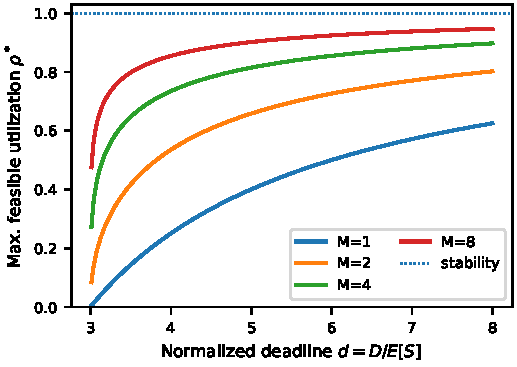
\includegraphics[width=\columnwidth]{../results/figures/icra/fig1_feasibility_frontier.pdf}
    \caption{Deadline-aware capacity versus ordinary stability. A stable system can still fail a deadline-constrained EHC target.}
    \label{fig:frontier}
\end{figure}

\subsection{Detector--capacity co-design}

\begin{figure}[t]
    \centering
    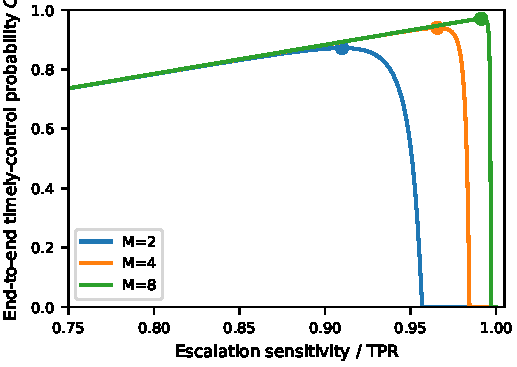
\includegraphics[width=\columnwidth]{../results/figures/icra/fig2_oversight_paradox.pdf}
    \caption{Oversight Paradox along a synthetic ROC curve. The EHC-maximizing operating point depends on supervisory capacity.}
    \label{fig:paradox}
\end{figure}

\subsection{False-positive scaling}

\begin{figure}[t]
    \centering
    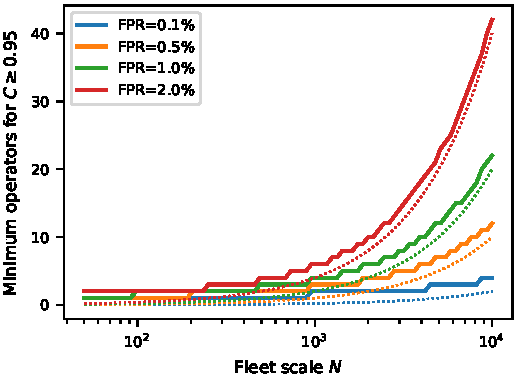
\includegraphics[width=\columnwidth]{../results/figures/icra/fig3_false_positive_scaling.pdf}
    \caption{Minimum staffing versus fleet scale for several false-positive rates, with first-order asymptotic slopes.}
    \label{fig:scaling}
\end{figure}

\subsection{Correlated demand and service-time robustness}

\begin{figure}[t]
    \centering
    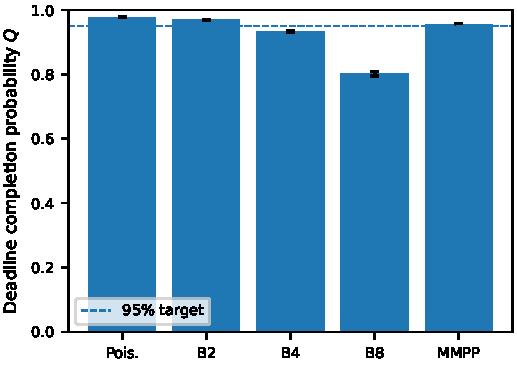
\includegraphics[width=\columnwidth]{../results/figures/icra/fig4_same_mean_burst.pdf}
    \caption{Identical mean offered load (\(\rho=0.4\)) under different temporal arrival structures.}
    \label{fig:burst}
\end{figure}

% Compress service-distribution robustness into a small panel or table if needed.

\section{Robotics Interpretation}
\label{sec:scenario}

We use variable-autonomy firefighting/search-and-rescue as a neutral interpretation: autonomous robots handle routine navigation and sensing while safety-critical or mission-sensitive contingencies can be referred to a human supervisor. Shared environmental changes naturally create correlated requests. Current HRI scales are used only to interpret the dimensionless axes; large fleets are explicitly scaling stress tests.

\section{Discussion and Limitations}
\label{sec:discussion}

The framework provides structural feasibility guarantees, not a universal cognitive model. Human correctness \(h\), intervention success \(a\), service-time distributions, event prevalence, and burst structure are application-specific and must ultimately be measured in the operational design domain. The analytical M/M/\(M\) assumptions are used for closed-form results; simulations test the main phenomena under non-exponential service and correlated arrivals.

The assurance implication is that human-in-the-loop should be evaluated as the performance of the complete escalation-and-supervision channel rather than as a binary architectural label.

\section{Conclusion}

A right or interface to intervene is not equivalent to an ability to intervene. Effective human control depends jointly on warning quality, scale, human capacity, deadlines, and temporal correlation.

\bibliographystyle{IEEEtran}
\bibliography{references}

\end{document}
